\documentclass[a4paper]{easychair}

\newenvironment{packed_itemize}{
\vspace*{-0.5em}
\begin{itemize}
  \setlength{\partopsep}{0pt}
  \setlength{\itemsep}{1pt}
  \setlength{\parskip}{0pt}
  \setlength{\parsep}{0pt}
}{\end{itemize}}

%\usepackage{amssymb}
\newcommand{\isa}{$\Rightarrow$}
\newcommand{\nta}{$\neg$}
\newcommand{\nra}{$\times$}
\newcommand{\xor}{$\oplus$}
\newcommand{\equ}{\textbullet}
%\newcommand{\isa}{{\em isa}}
%\newcommand{\nta}{{\em nota}}
%\newcommand{\nra}{{\em nvra}}
%\newcommand{\xor}{{\em xora}}

\begin{document}

\title{The SZS Ontologies for 
       Automated Reasoning Software}

\titlerunning{The SZS Ontologies}

\author{Geoff Sutcliffe \\
        {\footnotesize University of Miami}\\
        {\footnotesize Miami, USA}
}

\authorrunning{Geoff Sutcliffe}

\maketitle

%------------------------------------------------------------------------------
% Abstract
%
\begin{abstract}
This paper describes the SZS ontologies that provide status values for 
precisely describing what is known or has been established about logical data.
The ontology values are useful for describing existing logical data, and
for automated reasoning software to describe their input and output.
Standards for presenting the ontology values are also provided.
\end{abstract}

%------------------------------------------------------------------------------
\section{Introduction}
\label{Introduction}

The real use of automated reasoning software - automated theorem proving
(ATP) systems and other tools -
is not as standalone software that a user invokes directly, but rather
as embedded components of more complex reasoning systems.
For one example, NASA's certifiable program synthesis system \cite{DFS04-IJCAR}
embeds the SSCPA ATP system harness \cite{SS99-FLAIRS}, the ATP systems
E \cite{Sch02-AICOMM}, SPASS \cite{WS+07}, Vampire \cite{RV02-AICOMM},
and the GDV derivation verifier \cite{Sut06}.
For another example, SRI's BioDeducta system \cite{SW+07} embeds the
ATP system SNARK \cite{Sti-SNARK-URL}, and the BioBike integrated knowledge
base and biocomputing platform \cite{MT+05}.
In this embedded context automated reasoning software is typically
treated as a black box with known processing capabilities.
In order to use the software, the host system must know how to invoke the
software, how to pass data into the software, and how to accept data
produced by the software.

The data passed in to and out from automated reasoning software typically
consists of {\em logical data}, e.g., formulae, derivations, interpretations,
etc., and {\em status values} that describe what is known or has been
established about the logical data, e.g., the nature of the formulae, their
theoremhood or satisfiability, a reason why the software could not process
the data, etc.
For software that works with first-order logic, the de facto standard for
expressing logical data is the TPTP language \cite{SS+06} (and it is 
expected that this will soon extend to higher-order logic \cite{BRS08}).
The SZS ontologies that are linked to the TPTP are used by some automated
reasoning software to express the status values.
This paper describes the SZS ontologies and their use by automated reasoning
software.

The status information output by current automated reasoning software varies
widely in quantity, quality, and meaning.
At the low end of the scale, for example, an ATP system might report only
an assurance that the input problem's conjecture is a theorem of the axioms
(the wonderful ``{\tt yes}'' output).
In some cases the claimed status is misleading, e.g., when a clause normal form
refutation based ATP system claims that a first-order input problem consisting
of axioms and a conjecture is ``unsatisfiable'', it typically means that
the conjecture is a theorem of the axioms.
At the high end of the scale, for example, a tool such as Infinox might
report that a set of formulae does not have a finite model, or, for another
example, a set of formulae might be tagged as representing a Herbrand
interpretation.
In order to seamlessly embed automated reasoning software in more complex
reasoning systems, it is necessary to correctly and precisely specify status
values for the input and output data.
The SZS ontologies provide fine grained ontologies of status values
that are suitable for this task.

The SZS {\em success ontology} provides status values to describe what is 
known or has been successfully established about the relationship between 
the axioms and conjecture in logical data.
It is described in Section~\ref{Success}.
The SZS {\em no-success ontology} provides status values to describe why a
success ontology value has not been established.
It is described in Section~\ref{NoSuccess}.
The SZS {\em dataform ontology} provides status values to describe the nature
of logical data.
It is described in Section~\ref{Dataform}.
All status values are expressed as ``OneWord'' to make system output parsing
simple, and also have a three letter mnemonic.
In addition to the ontologies themselves, standards for {\em presenting
status values} have been specified.
These are described in Section~\ref{Presenting}.

%------------------------------------------------------------------------------
\section{The SZS Success Ontology}
\label{Success}

The SZS success ontology was inspired by work done to establish communication 
protocols for systems on the MathWeb Software Bus \cite{AKR00,ZK02}.
The ontology assumes that the logical data is a 2-tuple of the form
$\langle Ax, C \rangle$, where $Ax$ is a set (conjunction) of axioms and
$C$ is a conjecture formula.
This is a common standard usage of ATP systems.
If the input is not of the form $\langle Ax, C \rangle$, it is treated as
a conjecture formula (even if it is a ``set of axioms'' from the user view
point, e.g., a set of formulae all with the TPTP role {\tt axiom}), and
the 2-tuple is $\langle TRUE, C \rangle$.
The ontology values can also be interpreted in terms of the formula
$F \equiv Ax \Rightarrow C$.
The ontology values are based on the possible relationships
between the sets of models of $Ax$ and $C$.
For example, the ontology value {\tt Theorem} means that the set of models 
of $Ax$ is a (not necessarily strict) subset of the set of models of $C$, 
i.e., every model of $Ax$ is a model of $C$.
In this case $F$ is valid.

Figure~\ref{SuccessOntology} shows the success ontology (many of the
``OneWord'' status values are abbreviated in the figure - see
the list below for the official full ``OneWord''s).
The lines in the ontology can be followed up the hierarchy as
{\em isa} links, e.g., an ETH {\em isa} EQV {\em isa} (SAT and a THM).
% The dotted lines can be followed only once, e.g., a UCA {\em isa} UNC, but
% not a CSA (although a UCA {\em isa} SCC {\em isa} CAX {\em isa} CTH).
Figure~\ref{SuccessModels} shows the relationships between the model sets
for some of the success ontology values.
The outer grey ring contains all interpretations, the long dashed black
ring contains the models of $Ax$, and the short dashed black ring contains
the models of $C$.

\begin{figure}[htb]
  \begin{centering}
  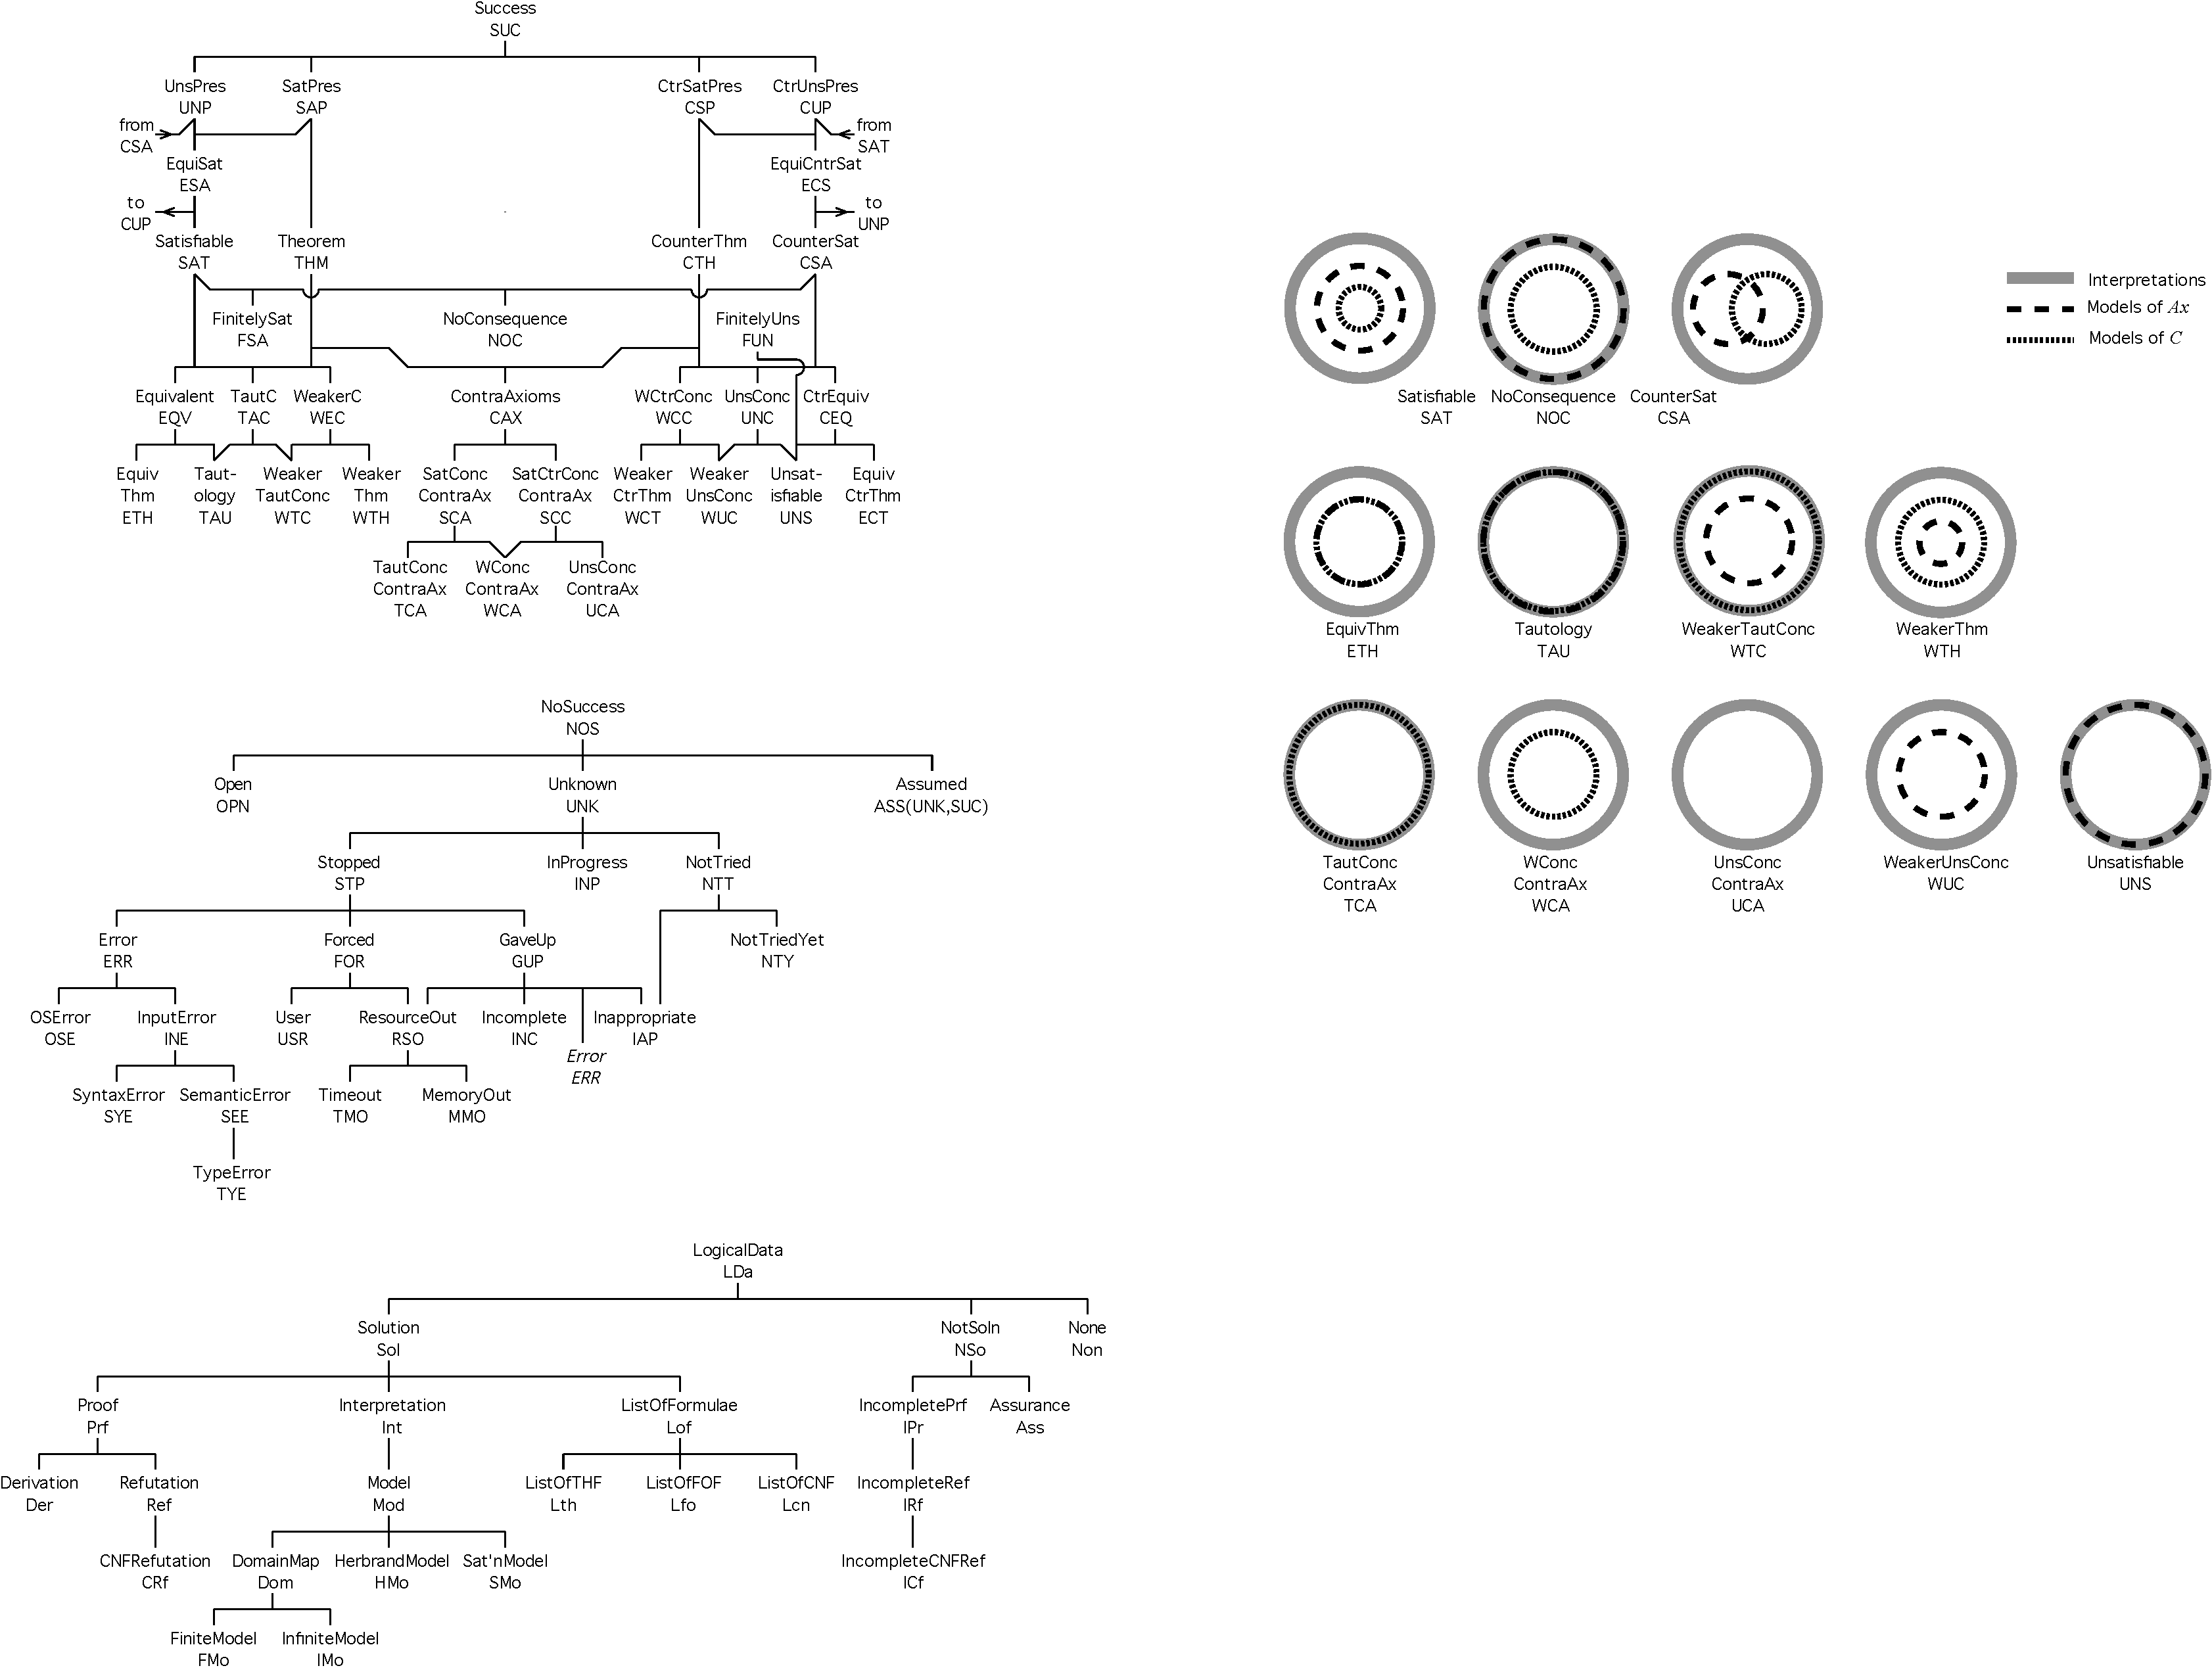
\includegraphics[width=0.75\textwidth]{Success}
  \caption{SZS Success Ontology}
  \label{SuccessOntology}
  \end{centering}
\end{figure}

\begin{figure}[htb]
  \begin{centering}
  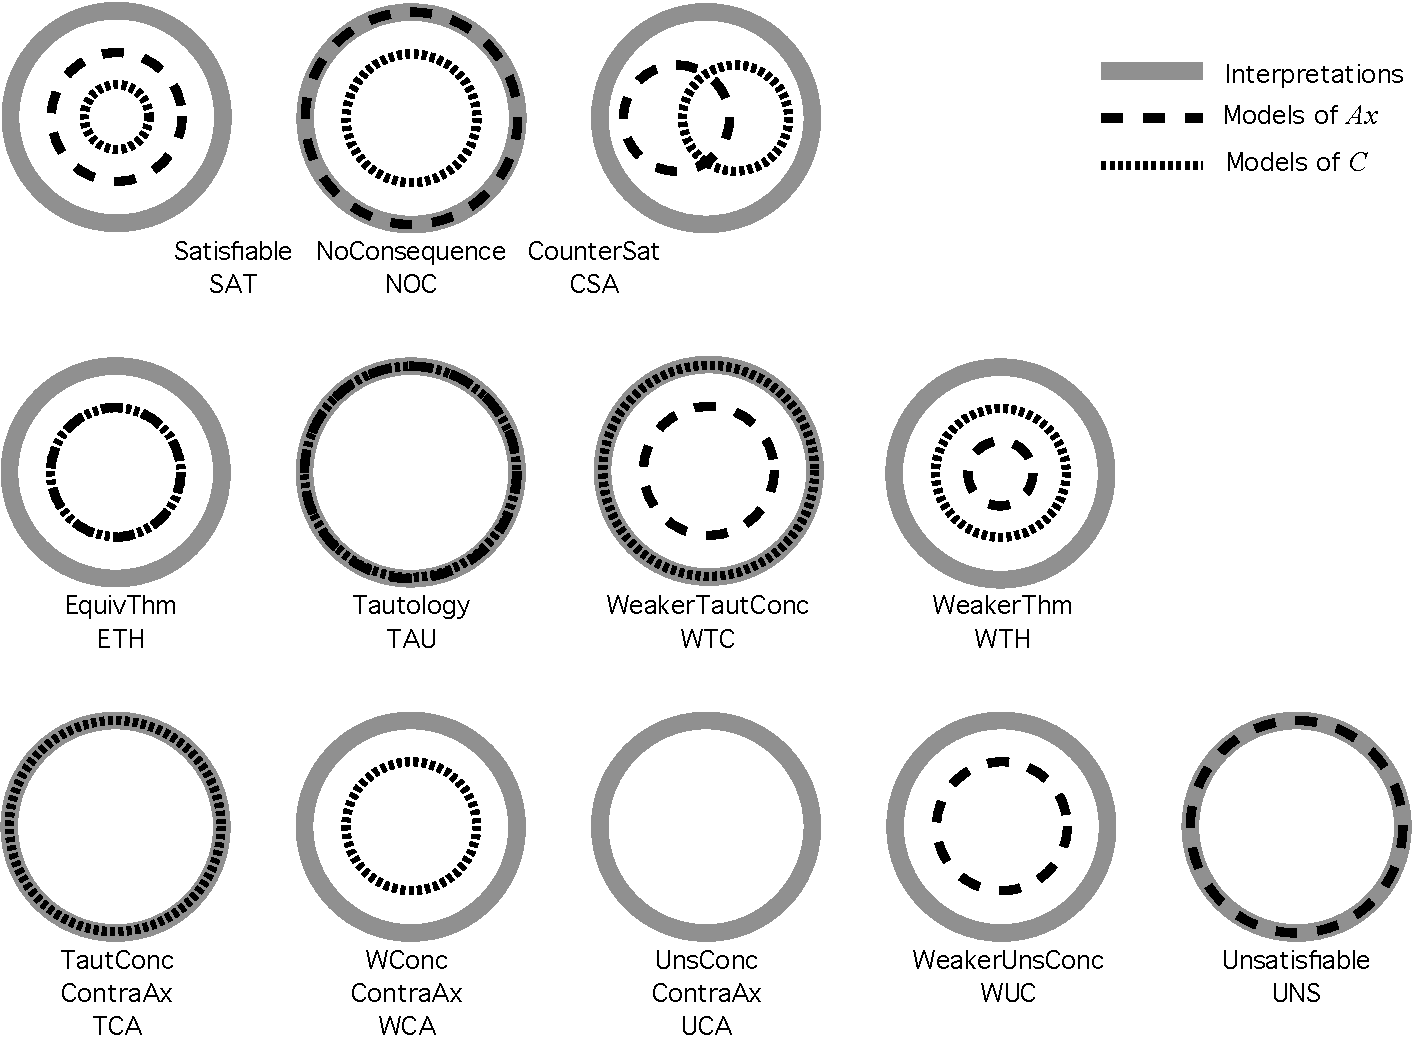
\includegraphics[width=0.6\textwidth]{SuccessModels}
  \caption{SZS Success Ontology Models}
  \label{SuccessModels}
  \end{centering}
\end{figure}

The meanings of the success ontology values are as follows.
Associated with each status value are some possible dataforms that might
be provided to justify the ontology value for given logical data -
see Section~\ref{Dataform}.

\begin{packed_itemize}
\item Success (SUC):
      The logical data has been processed successfully.

\item UnsatisfiabilityPreserving (UNP):
      If there does not exist a model of $Ax$ then there does not exist a
      model of $C$, i.e., if $Ax$ is unsatisfiable then $C$ is unsatisfiable.

\item SatisfiabilityPreserving (SAP):
      If there exists a model of $Ax$ then there exists a model of $C$, i.e.,
      if $Ax$ is satisfiable then $C$ is satisfiable.
      $F$ is satisfiable.

\item EquiSatisfiable (ESA):
      There exists a model of $Ax$ iff there exists a model of $C$, i.e.,
      $Ax$ is (un)satisfiable iff $C$ is (un)satisfiable.

\item Satisfiable (SAT):
      Some interpretations are models of $Ax$, and
      some models of $Ax$ are models of $C$.
      $F$ is satisfiable, and $\neg F$ is not valid.
      Possible dataforms are Models of $Ax \wedge C$.

\item FinitelySatisfiable (FSA):
      Some finite interpretations are finite models of $Ax$, and
      some finite models of $Ax$ are finite models of $C$.
      $F$ is satisfiable, and $\neg F$ is not valid.
      Possible dataforms are FiniteModels of $Ax \wedge C$.

\item Theorem (THM):
      All models of $Ax$ are models of $C$.
      $F$ is valid, and $C$ is a theorem of $Ax$.
      Possible dataforms are Proofs of $C$ from $Ax$.

\item Equivalent (EQV):
      Some interpretations are models of $Ax$,
      all models of $Ax$ are models of $C$, and
      all models of $C$ are models of $Ax$.
      $F$ is valid, $C$ is a theorem of $Ax$, and $Ax$ is a theorem of $C$.
      Possible dataforms are Proofs of $C$ from $Ax$ and of $Ax$ from $C$.

\item TautologousConclusion (TAC):
      Some interpretations are models of $Ax$, and
      all interpretations are models of $C$.
      $F$ is valid, and $C$ is a tautology.
      Possible dataforms are Proofs of $C$.

\item WeakerConclusion (WEC):
      Some interpretations are models of $Ax$,
      all models of $Ax$ are models of $C$, and
      some models of $C$ are not models of $Ax$.
      See Theorem and Satisfiable.

\item EquivalentTheorem (ETH):
      Some, but not all, interpretations are models of $Ax$,
      all models of $Ax$ are models of $C$, and
      all models of $C$ are models of $Ax$.
      See Equivalent.

\item Tautology (TAU):
      All interpretations are models of $Ax$, and
      all interpretations are models of $C$.
      $F$ is valid, $\neg F$ is unsatisfiable, and $C$ is a tautology.
      Possible dataforms are Proofs of $Ax$ and of $C$.

\item WeakerTautologousConclusion (WTC):
      Some, but not all, interpretations are models of $Ax$, and
      all interpretations are models of $C$.
      $F$ is valid, and $C$ is a tautology.
      See TautologousConclusion and WeakerConclusion.

\item WeakerTheorem (WTH):
      Some interpretations are models of $Ax$,
      all models of $Ax$ are models of $C$,
      some models of $C$ are not models of $Ax$, and
      some interpretations are not models of $C$.
      See Theorem and Satisfiable.

\item ContradictoryAxioms (CAX):
      No interpretations are models of $Ax$.
      $F$ is valid, and anything is a theorem of $Ax$.
      Possible dataforms are Refutations of $Ax$.

\item SatisfiableConclusionContradictoryAxioms (SCA):
      No interpretations are models of $Ax$, and
      some interpretations are models of $C$.
      See ContradictoryAxioms.

\item TautologousConclusionContradictoryAxioms (TCA):
      No interpretations are models of $Ax$, and
      all interpretations are models of $C$.
      See TautologousConclusion and SatisfiableConclusionContradictoryAxioms.

\item WeakerConclusionContradictoryAxioms (WCA):
      No interpretations are models of $Ax$, and
      some, but not all, interpretations are models of $C$.
      See SatisfiableConclusionContradictoryAxioms and 
      SatisfiableCounterConclusionContradictoryAxioms.

\item CounterUnsatisfiabilityPreserving (CUP):
      If there does not exist a model of $Ax$ then there does not exist a
      model of $\neg C$, i.e., if $Ax$ is unsatisfiable then $\neg C$ is
      unsatisfiable.

\item CounterSatisfiabilityPreserving (CSP):
      If there exists a model of $Ax$ then there exists a model of $\neg C$,
      i.e., if $Ax$ is satisfiable then $\neg C$ is satisfiable.

\item EquiCounterSatisfiable (ECS):
      There exists a model of $Ax$ iff there exists a model of $\neg C$, i.e.,
      $Ax$ is (un)satisfiable iff $\neg C$ is (un)satisfiable.

\item CounterSatisfiable (CSA):
      Some interpretations are models of $Ax$, and
      some models of $Ax$ are models of $\neg C$.
      $F$ is not valid, $\neg F$ is satisfiable, and $C$ is not a theorem
      of $Ax$.
      Possible dataforms are Models of $Ax \wedge \neg C$.

\item CounterTheorem (CTH):
      All models of $Ax$ are models of $\neg C$.
      $F$ is not valid, and $\neg C$ is a theorem of $Ax$.
      Possible dataforms are Proofs of $\neg C$ from $Ax$.

\item CounterEquivalent (CEQ):
      Some interpretations are models of $Ax$,
      all models of $Ax$ are models of $\neg C$, and
      all models of $\neg C$ are models of $Ax$
      (i.e., all interpretations are models of $Ax$ xor of $C$)
      $F$ is not valid, and $\neg C$ is a theorem of $Ax$.
      Possible dataforms are Proofs of $\neg C$ from $Ax$ and of $Ax$
      from $\neg C$.

\item UnsatisfiableConclusion (UNC):
      Some interpretations are models of $Ax$, and
      all interpretations are models of $\neg C$
      (i.e., no interpretations are models of $C$).
      F is not valid, and $\neg C$ is a tautology.
      Possible dataforms are Proofs of $\neg C$.

\item WeakerCounterConclusion (WCC):
      Some interpretations are models of $Ax$, and
      all models of $Ax$ are models of $\neg C$, and
      some models of $\neg C$ are not models of $Ax$.
      See CounterTheorem and CounterSatisfiable.

\item EquivalentCounterTheorem (ECT):
      Some, but not all, interpretations are models of $Ax$,
      all models of $Ax$ are models of $\neg C$, and
      all models of $\neg C$ are models of $Ax$.
      See CounterEquivalent.

\item FinitelyUnsatisfiable (FUN):
      All finite interpretations are finite models of $Ax$, and
      all finite interpretations are finite models of $\neg C$
      (i.e., no finite interpretations are finite models of $C$).

\item Unsatisfiable (UNS):
      All interpretations are models of $Ax$, and
      all interpretations are models of $\neg C$.
      (i.e., no interpretations are models of $C$).
      $F$ is unsatisfiable, $\neg F$ is valid, and $\neg C$ is a tautology.
      Possible dataforms are Proofs of $Ax$ and of $C$, and Refutations of $F$.

\item WeakerUnsatisfiableConclusion (WUC):
      Some, but not all, interpretations are models of $Ax$, and
      all interpretations are models of $\neg C$.
      See Unsatisfiable and WeakerCounterConclusion.

\item WeakerCounterTheorem (WCT):
      Some interpretations are models of $Ax$,
      all models of $Ax$ are models of $\neg C$,
      some models of $\neg C$ are not models of $Ax$, and
      some interpretations are not models of $\neg C$.
      See CounterSatisfiable.

\item SatisfiableCounterConclusionContradictoryAxioms (SCC):
      No interpretations are models of $Ax$, and
      some interpretations are models of $\neg C$.
      See ContradictoryAxioms.

\item UnsatisfiableConclusionContradictoryAxioms (UCA):
      No interpretations are models of $Ax$, and
      all interpretations are models of $\neg C$
      (i.e., no interpretations are models of $C$).
      See UnsatisfiableConclusion and 
      SatisfiableCounterConclusionContradictoryAxioms.

\item NoConsequence (NOC):
      Some interpretations are models of $Ax$,
      some models of $Ax$ are models of $C$, and
      some models of $Ax$ are models of $\neg C$.
      $F$ is not valid, $F$ is satisfiable, $\neg F$ is not valid,
      $\neg F$ is satisfiable, and $C$ is not a theorem of $Ax$.
      Possible dataforms are pairs of models, one Model of $Ax \wedge C$
      and one Model of $Ax \wedge \neg C$.

\end{packed_itemize}

The success ontology is very fine grained, and has more status values
than are commonly used by automated reasoning software, by ATP systems
in particular.
A suitable subset for practical uses of ATP systems is as follows:
\begin{packed_itemize}
\item FOF problems with a conjecture - report Theorem or CounterSatisfiable.
\item FOF problems without a conjecture - report Satisfiable or Unsatisfiable.
\item CNF problems - report Satisfiable or Unsatisfiable.
\end{packed_itemize}

%------------------------------------------------------------------------------
\subsection{Validation of the Success Ontology}
\label{Validation}

Two steps have been taken towards formal validation of the success
ontology.
The first step was the enumeration of the possible relationships between the
models of $Ax$ and $C$ (some of which are illustrated in
Figure~\ref{SuccessModels}).
This provided a basis for the ontology values, and a basis for the
{\em isa} links.
The second step\footnote{%
Thanks to the reviewer of this paper whose comments instigated this step.}
was to axiomatize the ontology and prove relevant properties.
(The axiomatization implemented covers the ``positive'' part of the
ontology regarding $Ax$ and $C$, and just two commonly used values from
the ``negative'' part regarding $Ax$ and$\neg C$.
It is expected that the results obtained will extend without difficulty
to the full ontology.)
The axiomatization encodes the relationship between the models of
$Ax$ and $C$ for each ontology value, and, from that, relationships
between the ontology values can be proven.
Additionally, a finite model of the axioms was found, demonstrating the
consistency of the axiomatization and hence the ontology.

The axiomatization is in first-order logic.
As example, the axioms that describe the ESA, THM, and ETH values are
given in Figure~\ref{Axioms}.
Four relationships between pairs of ontology values were defined and
axiomatized:
\begin{packed_itemize}
\item $\alpha$ {\em isa} $\beta$, meaning that if $\langle Ax, C \rangle$
      has the status $\alpha$ then it also has the status $\beta$.
      For example, WTH {\em isa} THM.
\item $\alpha$ {\em nota} $\beta$, meaning that if $\langle Ax, C \rangle$
      has the status $\alpha$ then it does not necessarily have the status
      $\beta$.
      For example, THM {\em nota} SAT (because SAT does not hold for
      the case of contradictory $Ax$).
\item $\alpha$ {\em nevera} $\beta$, meaning that if $\langle Ax, C \rangle$
      has the status $\alpha$ then it cannot have the status $\beta$.
      For example, SAT {\em nevera} CAX.
\item $\alpha$ {\em xora} $\beta$, meaning that every $\langle Ax, C \rangle$
      has the status $\alpha$ xor $\beta$.
      For example, THM {\em xora} CSA.
\end{packed_itemize}

Additionally, axioms that deal with properties of formulae and models were
provided.
The relationships and properties axioms are given in Figure~\ref{Axioms}.

\begin{figure}[htb]
  \begin{centering}
\begin{scriptsize}
\begin{verbatim}
fof(esa,axiom,(                      fof(thm,axiom,(                      fof(eth,axiom,(
    ! [Ax,C] :                           ! [Ax,C] :                           ! [Ax,C] :
      ( ( ? [I1] : model(I1,Ax)            ( ! [I1] :                           ( ( ? [I1] : model(I1,Ax)
      <=> ? [I2] : model(I2,C) )               ( model(I1,Ax)                     & ? [I2] : ~ model(I2,Ax)
    <=> status(Ax,C,esa) ) )).                => model(I1,C) )                    & ! [I1] :
                                         <=> status(Ax,C,thm) ) )).                   ( model(I1,Ax)
                                                                                      <=> model(I1,C) ) )
                                                                                <=> status(Ax,C,eth) ) )).

fof(isa,axiom,(                      fof(nota,axiom,(                     fof(nevera,axiom,(
    ! [S1,S2] :                          ! [S1,S2] :                          ! [S1,S2] :
      ( ! [Ax,C] :                         ( ? [Ax,C] :                         ( ! [Ax,C] :
          ( status(Ax,C,S1)                    ( status(Ax,C,S1)                    ( status(Ax,C,S1)
         => status(Ax,C,S2) )                  & ~ status(Ax,C,S2) )               => ~ status(Ax,C,S2) )
    <=> isa(S1,S2) ) )).                 <=> nota(S1,S2) ) )).                <=> nevera(S1,S2) ) )).

fof(xora,axiom,(                     fof(completeness,axiom,(             fof(not,axiom,(
    ! [S1,S2] :                          ! [I,F] :                            ! [I,F] :
      ( ! [Ax,C] :                         ( model(I,F)                         ( model(I,F)
          ( status(Ax,C,S1)              <~> model(I,not(F)) ) )).            <=> ~ model(I,not(F)) ) )).
        <~> status(Ax,C,S2) )
    <=> xora(S1,S2) ) )).

fof(tautology,axiom,(                fof(contradiction,axiom,(            fof(sat_non_taut_pair,axiom,(
    ? [F] : ! [I] : model(I,F) )).       ? [F] : ! [I] : ~ model(I,F) )).     ? [Ax,C] :
                                                                                ( ? [I1] :
fof(satisfiable,axiom,(              fof(non_thm_spt,axiom,(                        ( model(I1,Ax)
    ? [F] :                              ? [I1,Ax,C] :                              & model(I1,C) )
      ( ? [I1] : model(I1,F)               ( model(I1,Ax)                       & ? [I2] :
      & ? [I2] : ~ model(I2,F) ) )).       & ~ model(I1,C)                          ( ~ model(I2,Ax)
                                           & ? [I2] : model(I2,C) ) )).             | ~ model(I2,C) ) ) )).
\end{verbatim}
\end{scriptsize}
  \caption{SZS Success Ontology Axioms}
  \label{Axioms}
  \end{centering}
\end{figure}

The axiomatization was shown to be consistent by generating a finite
model using Paradox \cite{CS03}.
Some general properties of the relationships were proved using an ATP system
(see below for a discussion of the ATP system used), e.g., that {\em isa}
is a transitive relation, and that if $\alpha$ {\em isa} $\beta$ and
$\alpha$ {\em nota} $\gamma$ then $\beta$ {\em nota} $\gamma$.
Next the relationships between all pairs of ontology values were investigated,
using the ATP system to prove the relationships from the axioms.
The {\em isa} relationship was tested first, as if a pair of ontology
values has the {\em isa} relationship they cannot have any of the other three
relationships.
For those pairs that were not proved to have the {\em isa} relationship,
the {\em nevera} relationship was tested next.
For those pairs that were proved to have the {\em nevera} relationship the
{\em xora} relationship was tested, and for the other pairs the {\em nota}
relationship was tested.
Proving a {\em nota} relationship requires establishing the existence of 
formulae and models that deny the relationship.
In the axiomatization five examples are provided, the {\tt tautology},
{\tt satisfiable}, {\tt contradiction}, {\tt non\_thm\_spt} and 
{\tt sat\_non\_taut\_pair} axioms above.

The results of the testing are shown in Table~\ref{Relationships}, where
the vertical axis value has the shown relationship to the horizontal axis
value.
The {\em isa} relationship is denoted by \isa, {\em nota} by \nta,
{\em nevera} by \nra, and {\em xora} by \xor.
Sixty-eight pairs were proved to have the {\em isa} relationship,
89 to have the {\em nota} relationship,
179 to have the {\em nevera} (and not the {\em xora}) relationship,
4 to have the {\em xora} relationship, and
for the remaining two pairs no relationship could be proved.
The latter are the cases that WEC {\em nota} WTC and WEC {\em nota} TAC, 
which require exhibition of an $\langle Ax, C \rangle$ pair that has the 
WEC property but in which $C$ is not a tautology.
This could be done explicitly, along the lines of the 
{\tt sat\_non\_taut\_pair} axiom above, but that seemed like cheating.
Note that it is possible that some of the {\em nota} relationships might 
be {\em nevera}, and some of the {\em nevera} relationships might be 
{\em xora}, but could not be proved so.

As mentioned above, automated theorem proving was used to prove the
relationships between the ontology values.
At first, proofs were attempted using monolithic ATP systems such as EP, 
SPASS, and Vampire.
The success rate was low, because the axiomatization forms a
large theory - see \cite{SUS07}.
Therefore the SRASS system \cite{SP07} was used, and it was highly successful
in identifying the necessary axioms for proving each conjecture, and 
subsequently obtaining either a proof using EP or an assurance of a proof 
using iProver \cite{Kor08}.
In addition to SRASS, the MANSEX \cite{SYT09} and IDV \cite{TPS07}
tools were used during the initial development of the axiomatization, to
find the most obvious relationships and to analyze proofs.
All automated reasoning and proof processing was done on a computer with 
a Intel Xeon 2.80GHz CPU and 3GB memory, running the Linux 2.6 operating 
system, and with a 60s CPU time limit per proof attempt (on the entire SRASS 
process).

The formal analysis has had beneficial effects.
Three new ontology values were added,
three errors in the definitions of the ontology values were exposed and
corrected, four incorrect {\em isa} links in the ontology
were found and removed, and several unnoticed  {\em isa} relationships
were revealed and added.
The {\em isa} links in Figure~\ref{SuccessOntology} correspond to those
in Table~\ref{Relationships}.

\setlength{\tabcolsep}{2pt}
\begin{table}[bt]
\begin{center}
\begin{tabular}{l|ccccccccccccccccccc}
                    & {\footnotesize UNP} & {\footnotesize SAP} & {\footnotesize ESA} & {\footnotesize SAT} & {\footnotesize THM} & {\footnotesize EQV} & {\footnotesize TAC} & {\footnotesize WEC} & {\footnotesize ETH} & {\footnotesize TAU} & {\footnotesize WTC} & {\footnotesize WTH} & {\footnotesize CAX} & {\footnotesize SCA} & {\footnotesize TCA} & {\footnotesize WCA} & {\footnotesize CSA} & {\footnotesize UNS} & {\footnotesize NOC} \\
\hline
{\footnotesize UNP} &\equ &\nta &\nta &\nta &\nta &\nta &\nta &\nta &\nta &\nta &\nta &\nta &\nta &\xor &\nra &\nra &\nta &\nta &\nta \\
{\footnotesize SAP} &\nta &\equ &\nta &\nta &\nta &\nta &\nta &\nta &\nta &\nta &\nta &\nta &\nta &\nta &\nta &\nta &\nta &\nra &\nta \\
{\footnotesize ESA} &\isa &\isa &\equ &\nta &\nta &\nta &\nta &\nta &\nta &\nta &\nta &\nta &\nta &\nra &\nra &\nra &\nta &\nra &\nta \\
{\footnotesize SAT} &\isa &\isa &\isa &\equ &\nta &\nta &\nta &\nta &\nta &\nta &\nta &\nta &\nra &\nra &\nra &\nra &\nta &\nra &\nta \\
{\footnotesize THM} &\nta &\isa &\nta &\nta &\equ &\nta &\nta &\nta &\nta &\nta &\nta &\nta &\nta &\nta &\nta &\nta &\xor &\nra &\nra \\
{\footnotesize EQV} &\isa &\isa &\isa &\isa &\isa &\equ &\nta &\nra &\nta &\nta &\nra &\nra &\nra &\nra &\nra &\nra &\nra &\nra &\nra \\
{\footnotesize TAC} &\isa &\isa &\isa &\isa &\isa &\nta &\equ &\nta &\nra &\nta &\nta &\nra &\nra &\nra &\nra &\nra &\nra &\nra &\nra \\
{\footnotesize WEC} &\isa &\isa &\isa &\isa &\isa &\nra &\nta &\equ &\nra &\nra &\nta &\nta &\nra &\nra &\nra &\nra &\nra &\nra &\nra \\
{\footnotesize ETH} &\isa &\isa &\isa &\isa &\isa &\isa &\nra &\nra &\equ &\nra &\nra &\nra &\nra &\nra &\nra &\nra &\nra &\nra &\nra \\
{\footnotesize TAU} &\isa &\isa &\isa &\isa &\isa &\isa &\isa &\nra &\nra &\equ &\nra &\nra &\nra &\nra &\nra &\nra &\nra &\nra &\nra \\
{\footnotesize WTC} &\isa &\isa &\isa &\isa &\isa &\nra &\isa &\isa &\nra &\nra &\equ &\nra &\nra &\nra &\nra &\nra &\nra &\nra &\nra \\
{\footnotesize WTH} &\isa &\isa &\isa &\isa &\isa &\nra &\nra &\isa &\nra &\nra &\nra &\equ &\nra &\nra &\nra &\nra &\nra &\nra &\nra \\
{\footnotesize CAX} &\nta &\isa &\nta &\nra &\isa &\nra &\nra &\nra &\nra &\nra &\nra &\nra &\equ &\nta &\nta &\nta &\nra &\nra &\nra \\
{\footnotesize SCA} &\xor &\isa &\nra &\nra &\isa &\nra &\nra &\nra &\nra &\nra &\nra &\nra &\isa &\equ &\nta &\nta &\nra &\nra &\nra \\
{\footnotesize TCA} &\nra &\isa &\nra &\nra &\isa &\nta &\nra &\nra &\nra &\nra &\nra &\nra &\isa &\isa &\equ &\nra &\nra &\nra &\nra \\
{\footnotesize WCA} &\nra &\isa &\nra &\nra &\isa &\nra &\nra &\nra &\nra &\nra &\nra &\nra &\isa &\isa &\nra &\equ &\nra &\nra &\nra \\
{\footnotesize CSA} &\isa &\nta &\nta &\nta &\xor &\nra &\nra &\nra &\nra &\nra &\nra &\nra &\nra &\nra &\nra &\nra &\equ &\nta &\nta \\
{\footnotesize UNS} &\isa &\nra &\nra &\nra &\nra &\nra &\nra &\nra &\nra &\nra &\nra &\nra &\nra &\nra &\nra &\nra &\isa &\equ &\nra \\
{\footnotesize NOC} &\isa &\isa &\isa &\isa &\nra &\nra &\nra &\nra &\nra &\nra &\nra &\nra &\nra &\nra &\nra &\nra &\isa &\nra &\equ \\
\hline
\end{tabular}
\end{center}
\caption{Success Ontology Relationships}
\label{Relationships}
\end{table}
%------------------------------------------------------------------------------
\section{The SZS No-Success Ontology}
\label{NoSuccess}

While it is always hoped that automated reasoning software will successfully
process the logical data, and hence establish a success ontology value,
in reality this often does not happen, for a variety of reasons.
In order to understand and make productive use of a lack of success, e.g.,
\cite{MBI94,IB96}, it is necessary to precisely specify the reason for and
nature of the lack of success.
The SZS no-success ontology provides status values for describing the reasons.
Note that no-success is not the same as failure: failure means that the
software has completed its attempt to process the logical data and could not
establish a success ontology value.
In contrast, no-success might be because the software is still running, or
that it has not yet even started processing the logical data.
Figure~\ref{NoSuccessOntology} shows the no-success ontology.

\begin{figure}[htb]
  \begin{centering}
  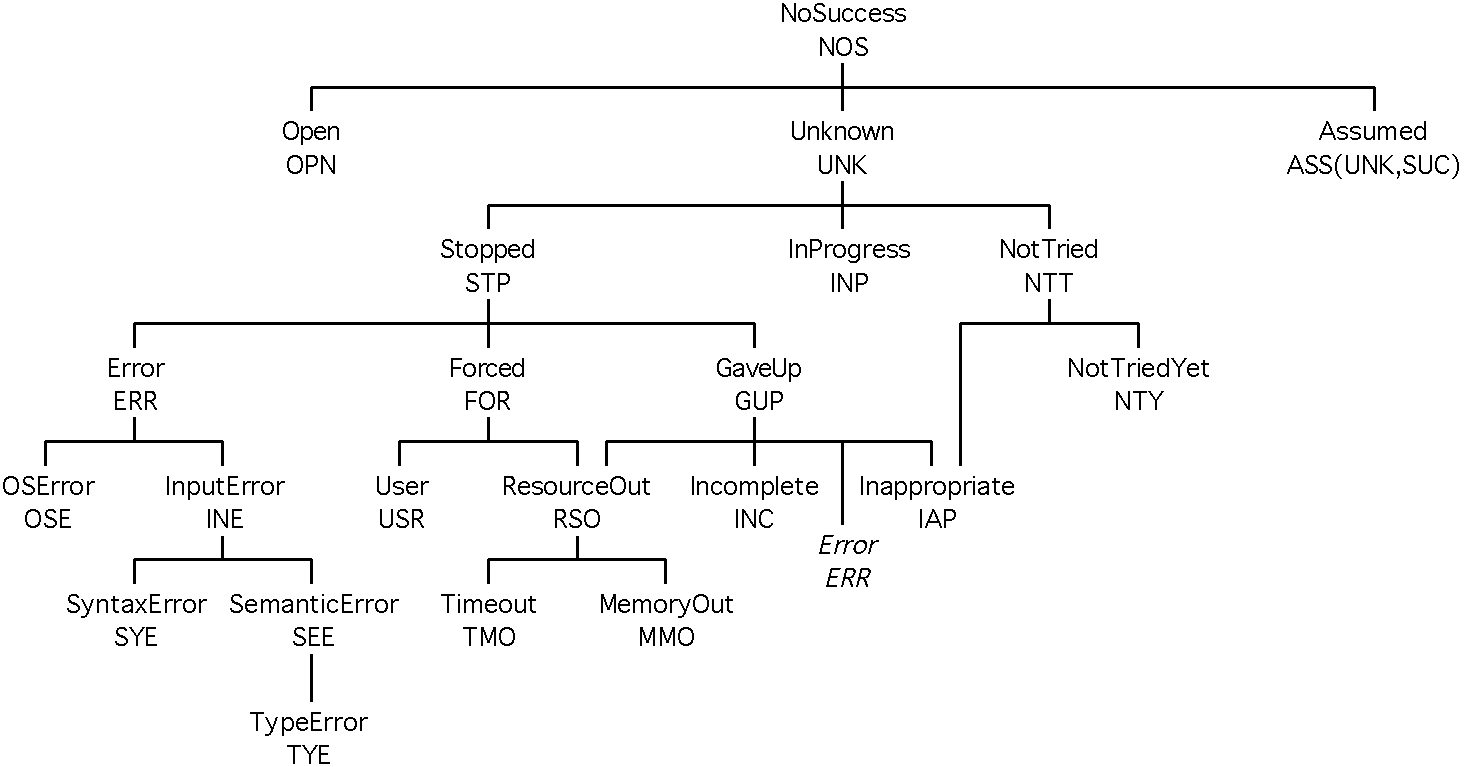
\includegraphics[width=0.85\textwidth]{NoSuccess}
  \caption{SZS No-Success Ontology}
  \label{NoSuccessOntology}
  \end{centering}
\end{figure}

The meanings of the no-success ontology values are as follows:
\begin{packed_itemize}
\item NoSuccess (NOS):
      The logical data has not been processed successfully (yet).

\item Open (OPN):
      A success value has never been established.

\item Unknown (UNK):
      Success value unknown, and no assumption has been made.

\item Assumed (ASS($U$,$S$)):
      The success ontology value $S$ has been assumed because the
      actual value is unknown for the no-success ontology reason $U$.
      $U$ is taken from the subontology starting at Unknown in the
      no-success ontology.

\item Stopped (STP):
      Software attempted to process the data, and stopped without a success
      status.

\item Error (ERR):
      Software stopped due to an error.

\item OSError (OSE):
      Software stopped due to an operating system error.

\item InputError (INE):
      Software stopped due to an input error.

\item SyntaxError (SYE):
      Software stopped due to an input syntax error.

\item SemanticError (SEE):
      Software stopped due to an input semantic error.

\item TypeError (TYE):
      Software stopped due to an input type error (for typed logical data).

\item Forced (FOR):
      Software was forced to stop by an external force.

\item User (USR):
      Software was forced to stop by the user.

\item ResourceOut (RSO):
      Software stopped because some resource ran out.

\item Timeout (TMO):
      Software stopped because the CPU time limit ran out.

\item MemoryOut (MMO):
      Software stopped because the memory limit ran out.

\item GaveUp (GUP):
      Software gave up of its own accord.

\item Incomplete (INC):
      Software gave up because it's incomplete.

\item Inappropriate (IAP):
      Software gave up because it cannot process this type of data.

\item InProgress (INP):
      Software is still running.

\item NotTried (NTT):
      Software has not tried to process the data.

\item NotTriedYet (NTY):
      Software has not tried to process the data yet, but might in the future.

\end{packed_itemize}

The no-success ontology is very fine grained, and has more status values
than are commonly used by automated reasoning software.
A suitable subset for practical uses is as follows:
\begin{packed_itemize}
\item The software stopped due to CPU limit - report Timeout.
\item The software gave up due to incompleteness - report GaveUp.
\item The software stopped due to an error - report Error.
\item Any other cases - report Unknown.
\end{packed_itemize}

%------------------------------------------------------------------------------
\section{The SZS Dataform Ontology}
\label{Dataform}

The success status values describe what is known or has been established
about the relationship between the axioms and conjecture in logical data,
but do not describe the form of logical data.
The dataform ontology provides suitable values for describing the
form of logical data.
The ontology values are commonly used to describe data provided
to justify a success ontology value, e.g., if an ATP system reports the
success ontology value {\tt Theorem} it might output a proof to justify that.
Figure~\ref{DataformOntology} shows the dataform ontology.

\begin{figure}[htb]
  \begin{centering}
  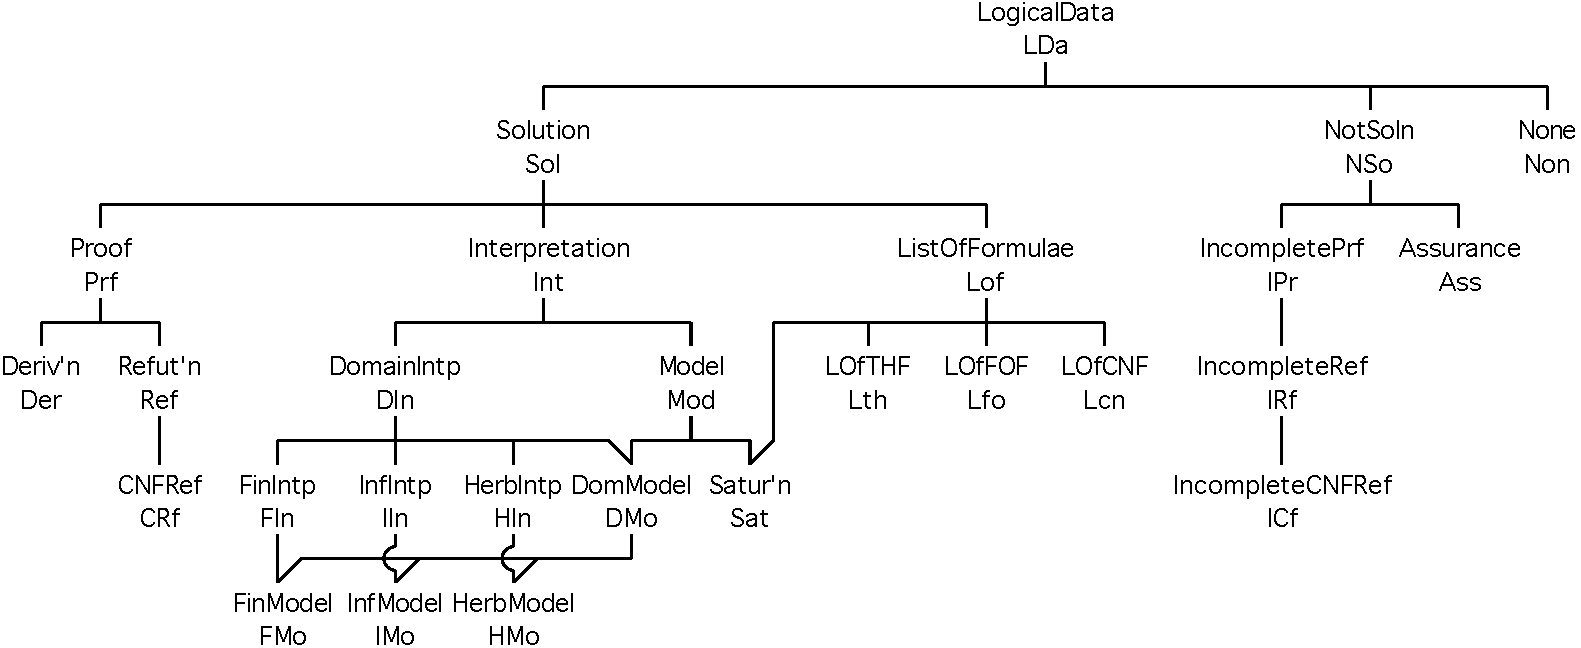
\includegraphics[width=\textwidth]{Dataform}
  \caption{SZS Dataform Ontology}
  \label{DataformOntology}
  \end{centering}
\end{figure}

The meanings of the dataform ontology values are as follows:
\begin{packed_itemize}
\item LogicalData (LDa):
      Logical data.

\item Solution (Sol):
      A solution.

\item Proof (Prf):
      A proof.

\item Derivation (Der):
      A derivation (inference steps ending in the theorem, in the
      Hilbert style).

\item Refutation (Ref):
      A refutation (starting with $Ax \cup \{\neg C\}$ and ending in FALSE).

\item CNFRefutation (CRf):
      A refutation in clause normal form, including, for FOF $Ax$ or $C$, 
      the translation from FOF to CNF (without the FOF to CNF translation
      it's an IncompleteRefutation).

\item Interpretation (Int):
      An interpretation.

\item DomainInterpretation (DIn):
      An interpretation expressed as a domain, a mapping for functions, 
      and a relation for predicates.

\item FiniteInterpretation (FIn):
      A domain interpretation with a finite domain.

\item InfiniteInterpretation (IIn):
      A domain interpretation with an infinite domain.

\item HerbrandInterpretation (HIn):
      A Herbrand interpretation.

\item Model (Mod):
      A model.

\item DomainModel (DMo):
      An model expressed as a domain, a mapping for functions, 
      and a relation for predicates.

\item FiniteModel (FMo):
      A domain model with a finite domain.

\item InfiniteModel (IMo):
      A domain model with an infinite domain.

\item HerbrandModel (HMo):
      A Herbrand model.

\item Saturation (Sat):
      A model expressed as a saturating set of formulae.

\item ListofFormulae (Lof):
      A list of formulae.

\item ListofTHF (Lth):
      A list of THF formulae.

\item ListofFOF (Lfo):
      A list of FOF formulae.

\item ListofCNF (Lcn):
      A list of CNF formulae.

\item IncompleteProof (IPr):
      A proof with part missing.

\item IncompleteRefutation (IRf):
      A refutation with parts missing.

\item IncompleteCNFRefutation (ICf):
      A CNF refutation with parts missing.

\item Assurance (Ass):
      Only an assurance of the success ontology value.

\item None (Non):
      Nothing.

\end{packed_itemize}

The dataform ontology is very fine grained, and has more status values
than are commonly used by automated reasoning software, by ATP systems
in particular.
A suitable subset for practical uses of ATP systems is as follows:
\begin{packed_itemize}
\item A generic proof - report Proof.
\item A refutation - report Refutation.
\item A CNF refutation - report CNFRefutation.
\item A generic model - report Model.
\item A finite model - report FiniteModel.
\item A Herbrand model - report HerbrandModel.
\item A saturation model - report SaturationModel.
\end{packed_itemize}

%------------------------------------------------------------------------------
\section{The SZS Presentation Standards}
\label{Presenting}

The SZS ontologies provide status values that precisely describe what is
known or has been established about logical data.
In order to make the use of the values easy in more complex reasoning
systems, it is necessary to specify precisely how the values should be
presented.
This makes it easy for harness software to prepare input data and examine
output data that contains ontology values, e.g., in practice, to {\tt grep}
the output from automated reasoning software for lines that provide status
values.

Success and no-success ontology values should be presented in lines of
the form

{\tt \% SZS status} {\em (no-)success\_ontology\_value} {\tt for} {\em logical\_data\_identifier}\\
(The leading '{\tt \%}' makes the line into a TPTP language comment.)
For examples

{\tt \% SZS status Unsatisfiable for SYN075+1}

{\tt \% SZS status GaveUp for SYN075+1}\\

A success or no-success ontology value should be presented as early as 
possible, at least before any data output to justify the value.
The justifying data should be delimited by lines of the form

{\tt \% SZS output start} {\em dataform\_ontology\_value} {\tt for} {\em logical\_data\_identifier}\\
and

{\tt \% SZS output end} {\em dataform\_ontology\_value} {\tt for} {\em logical\_data\_identifier}\\
For example

{\tt \% SZS output start CNFRefutation for SYN075-1}

{\tt ~~~~}{\em output\_logical\_data}

{\tt \% SZS output end CNFRefutation for SYN075-1}\\

All ``SZS'' lines can optionally have software specific information
appended, separated by a {\tt :}, i.e.,

{\tt \% SZS status} {\em (no-)success\_ontology\_value} {\tt for} {\em logical\_data\_id} {\tt :} {\em software\_specific\_information}

{\tt \% SZS output start} {\em dataform\_ontology\_value} {\tt for} {\em logical\_data\_id} {\tt :} {\em software\_specific\_info}

{\tt \% SZS output end} {\em dataform\_ontology\_value} {\tt for} {\em logical\_data\_id} {\tt :} {\em software\_specific\_info}\\
For examples

{\tt \% SZS status GaveUp for SYN075+1 :~Could not complete CNF conversion}

{\tt \% SZS output end CNFRefutation for SYN075-1 :~Completed in CNF conversion}

%------------------------------------------------------------------------------
\section{Conclusion}
\label{Conclusion}

This paper has presented the SZS ontologies of status values that are 
suitable for expressing precisely what is known or has been established 
about logical data.
The ontologies can be used for existing logical data, e.g., they are used
for the status of problems in the TPTP problem library \cite{SS98-JAR} and
solutions in the TSTP solution library \cite{Sut-TSTP-URL}, and can be used by
automated reasoning software to describe their input and output.
Already several ATP systems, e.g., Darwin \cite{BFT04}, E, Metis \cite{Hur03},
Paradox \cite{CS03}, use the SZS ontologies and the presentation standards,
and this contributes to simplifying their embedding into more complex
reasoning systems.

In addition to its use for reporting the overall status of a
$\langle Ax, C \rangle$ 2-tuple, the SZS success ontology is used
to report the status of individual inference steps in TPTP format
derivations \cite{SS+06}.
This is done in the ``useful information'' field of an {\tt inference}
record of an inferred formula.
For example, in
\begin{verbatim}
cnf(58,plain,
    ( ~ hates(agatha,esk2_1(butler)) ),
    inference(spm,[status(thm)],[51,48])).
\end{verbatim}
the status is Theorem (recorded as a lowercase acronym value {\tt thm}),
which indicates that the formulae is a theorem of it's two parent formulae
{\tt 51} and {\tt 48}.
The Theorem status is most common in derivations, but the SAP and ESA status
values are also used quite often, e.g., for the formulae inferred by
Skolemization and splitting steps.
These status values can be used for semantic verification of the derivations,
as is done by the GDV derivation verifier \cite{Sut06}.

While the SZS ontologies are in use and have matured to some extent, it
is not claimed that they are comprehensive and perfect.
Developers and users of automated reasoning software are invited to provide
feedback that might lead to improvements and increased usage.
Already some users are working on success ontology values for results from
computer algebra and other computational reasoning systems.
In related work, SZS standards for returning answers from question-and-answer
systems have been proposed.\footnote{%
See \url{http://www.tptp.org/TPTP/Proposals/AnswerExtraction.html}}
It is hoped that over time, with increased usage, the ontologies will
become battle hardened, and will be a core standard for automated reasoning.

%------------------------------------------------------------------------------
\bibliographystyle{plain}
\bibliography{Bibliography.bib}
%------------------------------------------------------------------------------
\end{document}
%------------------------------------------------------------------------------
